\section{Eksperimen dengan hardware (FPGA)}

\subsection{Pengenalan IO}

{\color{red} Perlu gambar board FPGA yang akan digunakan}

Beberapa daftar port dari board FPGA yang digunakan:

\begin{table}[H]
\caption{Beberapa port yang digunakan pada board FPGA}\label{tab:pin}
\centering
\begin{tabular}{|c|c|}
\hline 
Clock & PIN\_23\\
\hline 
Reset Push Button & PIN\_25\\
\hline 
Buzzer & PIN\_110 \\
\hline
IR & PIN\_100 \\
\hline 
\multicolumn{2}{|c|}{Push Button}\\
\hline 
key1 & PIN\_88 \\
\hline 
key2 & PIN\_89 \\
\hline 
key3 & PIN\_90 \\
\hline 
key4 & PIN\_91 \\
\hline 
\multicolumn{2}{|c|}{LED} \\
\hline 
LED1 & PIN\_87 \\
\hline 
LED2 & PIN\_86 \\
\hline 
LED3 & PIN\_85 \\
\hline 
LED4 & PIN\_84 \\
\hline 
\end{tabular}
\par
\end{table}



Untuk PIN assignment, buat skematik atau file Verilog terlebih dahulu, kemudian compile.
Buka PIN assignment, set pin yang diperlukan.

Prosedur ini diberikan pada contoh menyalakan LED.

\subsubsection{LED}

Buat project baru dengan nama {\sf led\_light},
misalnya. Kemudian tambahkan file Verilog berikut
ke project. Kode Verilog ini memberikan nilai logika ke tiap
LED (hardwired, tanpa ada input).

{\setstretch{1.0}
\begin{verilogcode}
module led_light(led);
  output[3:0] led;
  assign led = 4'b0000; // coba ubah-ubah nilai ini untuk tiap LED
endmodule
\end{verilogcode}
}

Compile file ini dengan cara klik icon {\sf Compile} atau dengan menu
{\sf Processing -> Start Compilation} atau menggunakan shortcut
{\sf Ctrl + L}.

Jika tidak ada kesalahan pada saat proses kompilasi,
maka langkah selanjutnya adalah melakukan
PIN assignment, yang dapat dilakukan dengan memilih menu
{\sf Assignment -> Pin Planner} atau menggunakan shortcut
{\sf Ctrl + N}. Atur PIN assigment sesuai dengan Tabel \ref{tab:pin}.

\begin{figure}[H]
\centering
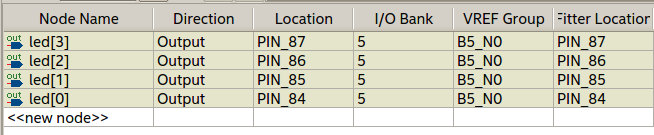
\includegraphics[scale=0.5]{images/PinPlanner_4LED.png}
\par
\caption{PIN Assignment untuk 4 LED}
\end{figure}

Compile lagi file tersebut.

Jika tidak ada pesan error, langkah selanjutnya adalah mendownload program
ini ke FPGA. Proses ini dapat dilakukan dengan cara memilih menu
{\sf Tools -> Programmer}.
Klik button {\sf Add File} untuk menambahkan file {\sf led\_light.sof}.
File ini biasanya ada di dalam subdirektori {\sf output} dari direktori
project.
Pastikan juga hardware terdeteksi. Jika belum terdeteksi, tambahkan melalui
dengan mengklik button {\sf Hardware Setup}.

\begin{figure}[H]
\centering
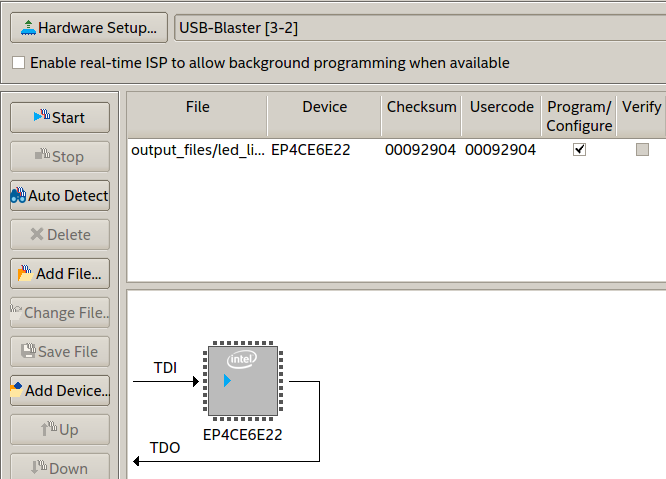
\includegraphics[scale=0.6]{images/Programmer_4LED.png}
\par
\caption{Tampilan tool {\sf Programmer}}
\end{figure}

\textbf{Catatan}

Pada board FPGA yang digunakan urutan LED dari kiri ke kanan adalah LED1,
LED2, LED3, dan LED4.
Misalkan memberikan assignment sebagai berikut.
\begin{itemize}
\item LED1 diwakili dengan {\tt led[0]}
\item LED2 diwakili dengan {\tt led[1]}
\item LED3 diwakili dengan {\tt led[2]}
\item LED4 diwakili dengan {\tt led[3]}
\end{itemize}
Misalkan juga kita memberikan nilai logika pada {\tt led} dengan
kode Verilog berikut.
\begin{verilogcode}
  led = 4'b1010;
\end{verilogcode}
Maka nilai 0 (nilai bit paling kanan atau LSB) diberikan pada {\tt led[0]}
atau LED1. Nilai pada bit kedua dari kanan diberikan untuk {\tt led[1]}, bit ketiga
untuk {\tt led[2]}, dan bit keempat (paling kiri atau MSB) untuk {\tt led[3]}.

Bagian {\sf output [3:0] led} pada kode di atas dapat diganti
dengan {\sf output [1:4] led} untuk memudahkan assignment nilai logika
sesuai dengan urutan LED di board yang digunakan. Sehingga kita dapat
melakukan assigment sebagai berikut.
\begin{itemize}
\item LED1 diwakili dengan {\tt led[1]}
\item LED2 diwakili dengan {\tt led[2]}
\item LED3 diwakili dengan {\tt led[3]}
\item LED4 diwakili dengan {\tt led[4]}
\end{itemize}

Cobalah bereksprimen dengan cara mengganti-ganti nilai logika
dari {\tt led}, kemudian isilah tabel berikut.

\begin{table}[H]
\centering
\begin{tabular}{|c|c|}
\hline
Nilai logika & Keadaan LED (on/off) \\
\hline
0 & \\
1 & \\
\hline
\end{tabular}
\par
\end{table}


\subsubsection{Push buttons}

Buat project baru, dan buat file Verilog dengan mendefiniskan satu modul
dengan input dari push button dan output ke LED.
\begin{verilogcode}
module test_buttons( buttons, led );
  input  [3:0] buttons;
  output [3:0] led;

  assign led = buttons;
endmodule
\end{verilogcode}

Bisa juga menggunakan potongan kode berikut.
\begin{verilogcode}
  assign led[0] = buttons[0];
  assign led[1] = buttons[1];
  assign led[2] = buttons[2];
  assign led[3] = buttons[3];
\end{verilogcode}

Cobalah bereksperimen dengan kode Verilog yang ada dan juga menggukan operator Verilog
seperti 

\begin{table}[H]
\centering
\begin{tabular}{|c|c|}
\hline
Nilai logika & Keadaan PB \\
\hline
0 & \\
1 & \\
\hline
\end{tabular}
\par
\end{table}

\subsubsection{Seven segments}

Lihat Modul 1.

\subsubsection{Clock}
{\color{red} Berapa frekuensi clock yang digunakan ? 50 MHz ?}

LED blinking (sudah menggunakan counter, implementasinya
mudah pada Verilog)

\subsubsection{IR}
Menggunakan protokol NEC.

Ubah kode Verilog yang sudah ada menjadi blok yang menampilkan

\subsection{Rangkaian kombinasional}

- rangkaian pendeteksi genap ganjil, input 4 PB, output 1 LED

- Input PB -> BCD -> seven segment

- IR -> BCD -> seven segment

- Implementasi XOR

- half adder dan full adder

- Menyalakan satu atau beberapa LED dengan kombinasi input
4 push button yang diberikan.
\begin{itemize}
\item LED1 menyala jika button1 dan button3 ditekan atau button1 dan button 4 ditekan
\item LED2 menyala jika button2 dan button4 ditekan atau button1 ditekan
\end{itemize}

- Input BCD (dari ) ke output seven segment. Buat tabel kebenaran dan rangkaian (dalam skematik
atau Verilog struktural).

{\centering
\begin{tabular}{|c|c|c|c||c|c|c|c|c|c|c|c|}
\hline
\multicolumn{4}{|c||}{Input} & \multicolumn{8}{|c|}{Output} \\
\hline
PB1 & PB2 & PB3 & PB4 & a & b & c & d & e & f & g & dp \\
\hline
0 & 0 & 0 & 0 &  &  &  &  &  &  &  & \\
0 & 0 & 0 & 1 &  &  &  &  &  &  &  & \\
0 & 0 & 1 & 0 &  &  &  &  &  &  &  & \\
... & ... & ... & ... &  &  &  &  &  &  &  & \\
1 & 1 & 1 & 1 &  &  &  &  &  &  &  & \\
\hline
\end{tabular}
\par}


\subsection{Rangkaian sekuensial}

- Implementasi D flip-flop

- Implementasi J-K flip-flop dan

- Implementasi T flip-flip. Toggle operation: buzzer dan LED

- register, counter

- Kalkulator sederhana, input dari remote IR ?

- Rangkaian multiplexing LED

- Menampilkan LED perdigit


